\documentclass[12pt,a4paper]{standalone}
\usepackage{amssymb}
\usepackage{amsmath}
\usepackage{bm}
\usepackage{tikz}
\usetikzlibrary{arrows.meta}
\usetikzlibrary{arrows}
\usepackage{pstricks}
\usetikzlibrary{patterns}
\usetikzlibrary{fadings}
\usetikzlibrary{shapes.geometric}


\begin{document}
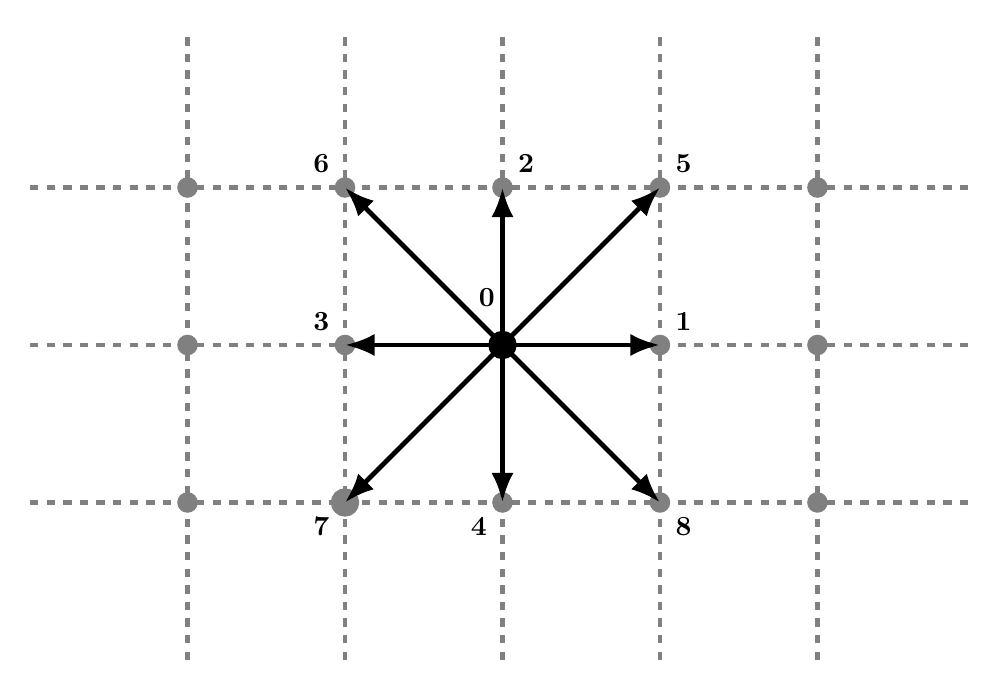
\begin{tikzpicture}[line width=0.6mm]
    %\draw [dashed,line width=0.5mm] (0,0) rectangle(12,8);
    \draw[gray,dashed,thick,line width=0.6mm] (0,2) -- (12,2);
    \draw[gray,dashed,thick,line width=0.6mm] (0,4) -- (12,4);
    \draw[gray,dashed,thick,line width=0.6mm] (0,6) -- (12,6);
    \draw[gray,dashed,thick,line width=0.6mm] (2,0) -- (2,8);
    \draw[gray,dashed,thick,line width=0.6mm] (4,0) -- (4,8);
    \draw[gray,dashed,thick,line width=0.6mm] (6,0) -- (6,8);
    \draw[gray,dashed,thick,line width=0.6mm] (8,0) -- (8,8);
    \draw[gray,dashed,thick,line width=0.6mm] (10,0) -- (10,8);

    \draw[black,fill=black] (6,4)node[]{} circle(0.15cm);
    \draw[gray,fill=gray] (2,2)node[]{} circle(0.1cm);
    \draw[gray,fill=gray] (4,2)node[]{} circle(0.15cm);
    \draw[gray,fill=gray] (6,2)node[]{} circle(0.1cm);
    \draw[gray,fill=gray] (8,2)node[]{} circle(0.1cm);
    \draw[gray,fill=gray] (10,2)node[]{} circle(0.1cm);

    \draw[gray,fill=gray] (2,4)node[]{} circle(0.1cm);
    \draw[gray,fill=gray] (4,4)node[]{} circle(0.1cm);
    %\draw[black,fill=black] (6,4)node[]{} circle(0.15cm);
    \draw[gray,fill=gray] (8,4)node[]{} circle(0.1cm);
    \draw[gray,fill=gray] (10,4)node[]{} circle(0.1cm);

    \draw[gray,fill=gray] (2,6)node[]{} circle(0.1cm);
    \draw[gray,fill=gray] (4,6)node[]{} circle(0.1cm);
    \draw[gray,fill=gray] (6,6)node[]{} circle(0.1cm);
    \draw[gray,fill=gray] (8,6)node[]{} circle(0.1cm);
    \draw[gray,fill=gray] (10,6)node[]{} circle(0.1cm);

    \draw[-Latex,shorten <=-2pt,solid,line width=0.6mm] (6,4) -- (8,4); %1
    \draw[-Latex,shorten <=-2pt,solid,line width=0.6mm] (6,4) -- (4,4); %3
    \draw[-Latex,shorten <=-2pt,solid,line width=0.6mm] (6,4) -- (6,6); %2
    \draw[-Latex,shorten <=-2pt,solid,line width=0.6mm] (6,4) -- (6,2); %4
    \draw[-Latex,shorten <=-2pt,solid,line width=0.6mm] (6,4) -- (8,6); %5
    \draw[-Latex,shorten <=-2pt,solid,line width=0.6mm] (6,4) -- (4,6); %5
    \draw[-Latex,shorten <=-2pt,solid,line width=0.6mm] (6,4) -- (4,2); %7
    \draw[-Latex,shorten <=-2pt,solid,line width=0.6mm] (6,4) -- (8,2); %8

    % \draw[white,fill=white] (6,4)node[]{} circle(0.3cm);
    % \draw (6,4) circle [radius=0.3] node {$\mathbf{0}$};
    \draw (5.8,4.6)node[]{$\mathbf{0}$};
    \draw (8.3,4.3)node[]{$\mathbf{1}$};
    \draw (6.3,6.3)node[]{$\mathbf{2}$};
    \draw (3.7,4.3)node[]{$\mathbf{3}$};
    \draw (5.7,1.7)node[]{$\mathbf{4}$};
    \draw (8.3,6.3)node[]{$\mathbf{5}$};
    \draw (3.7,6.3)node[]{$\mathbf{6}$};
    \draw (3.7,1.7)node[]{$\mathbf{7}$};
    \draw (8.3,1.7)node[]{$\mathbf{8}$};

    % \draw (7.5,4.3)node[]{$\mathbf{f_1}$};
    % \draw (5.7,5.5)node[]{$\mathbf{f_2}$};
    % \draw (4.5,3.7)node[]{$\mathbf{f_3}$};
    % \draw (6.3,2.5)node[]{$\mathbf{f_4}$};
    % \draw (7.1,5.5)node[]{$\mathbf{f_5}$};
    % \draw (4.4,5.2)node[]{$\mathbf{f_6}$};
    % \draw (4.8,2.3)node[]{$\mathbf{f_7}$};
    % \draw (7.6,2.8)node[]{$\mathbf{f_8}$};
\end{tikzpicture}
\end{document}

